\begin{center}KUGELFUNKTIONEN.\end{center}
\begin{center}[1.]\end{center}
Das folgende Verfahren zerlegt $P$, \textit{eine homogene Funktion} von $x,y,z$ der Ordnung $i$, in \textit{reine Kugelfunktionen}.

Man setze
\[
\frac{\mathrm d\mathrm dP}{\mathrm dx^2}+\frac{\mathrm d\mathrm dP}{\mathrm dy^2}+\frac{\mathrm d\mathrm dP}{\mathrm dz^2}=P'=fP,\quad fP'=P'',\quad fP''=fP''',\ \text{etc.}
\]
und schreibe der Kürze halber $xx+yy+zz=\rho$. Man bringt dann $P$ in die Form
\[
P=A+\rho B+\rho\rho C+\rho^3D+\text{usw.}
\]
sodass $A$, $B$, $C$, $D$ usw. reine Kugelfunktionen sind. Dazu dienen die folgenden Gleichungen
\SourceLeaf{637}
\[
\begin{aligned}
P&=A+\rho B+\rho\rho C+\rho^3D+\rho^4E+\text{usw.}\\
P'&=2(2i-1)B+4(2i-3)\rho C+6(2i-5)\rho\rho D\\
&\qquad+8(2i-7)\rho^3E+\text{usw.}\\
P''&=2.4(2i-3)(2i-5)C+4.6(2i-5)(2i-7)\rho D\\
&\qquad+6.8(2i-7)(2i-9)\rho\rho E+\text{usw.}\\
P'''&=2.4.6(2i-5)(2i-7)(2i-9)D\\
&\qquad+4.6.8(2i-7)(2i-9)(2i-11)\rho E+\text{usw.}\\
P''''&=2.4.6.8(2i-7)(2i-9)(2i-11)(2i-13)E+\text{usw.}
\end{aligned}
\]

Man kann diese Gleichungen auch anders darstellen, indem man die in $\rho\, .\, .\, .\,RR$ angegebene Ersetzung vornimmt und bei den Differentiationen nur $R$ als veränderlich betrachtet.
\[
\frac{\mathrm d\mathrm d.R^{-i}P}{\mathrm dR^2}+R^{-i}.P'=i(i+1).R^{-i-2}P
\]

\begin{center}[2.]\\\textit{Geometrische Bedeutung der Kugelfunktionen.}\end{center}
$P$ ist der unbestimmte Punkt.

$A$, $B$, $C$, $D$ usw. sind festgelegte Punkte.

Kugelfunktion erster Ordnung $\alpha\cos PA$

Zweite Ordnung
\[
\alpha\cos PA.\cos PC+\beta\cos PB.\cos PD
\]
wobei sich $A$, $B$, $C$, $D$ auf vier Flächen eines regelmäßigen Oktaeders beziehen.
\begin{center}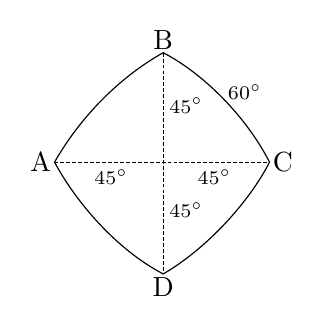
\begin{tikzpicture}[x=1cm,y=1cm,line width=.42pt,inner sep=1pt]
  \coordinate (A) at (-1.38,0);
  \coordinate (B) at (0,1.39);
  \coordinate (C) at (1.35,0);
  \coordinate (D) at (0,-1.42);
  \draw (A) .. controls (-1.06,.56) and (-.57,1.07) .. (B)
            .. controls (.52,1.12) and (1.06,.57) .. (C)
            .. controls (1.09,-.51) and (.55,-1.10) .. (D)
            .. controls (-.59,-1.11) and (-1.10,-.52) .. (A) -- cycle;
  \draw[dash pattern=on 1.4pt off .75pt] (A) -- (C) (B) -- (D);
  \node[left]  at (A) {$\mathrm A$};
  \node[above] at (B) {$\mathrm B$};
  \node[right] at (C) {$\mathrm C$};
  \node[below] at (D) {$\mathrm D$};
  \node[anchor=west]  at (.035,.72)  {\scriptsize $45^\circ$};
  \node[anchor=west]  at (.035,-.61) {\scriptsize $45^\circ$};
  \node[anchor=north] at (-.66,-.05) {\scriptsize $45^\circ$};
  \node[anchor=north] at (.65,-.05)  {\scriptsize $45^\circ$};
  \node[anchor=west]  at (.78,.89)   {\scriptsize $60^\circ$};
\end{tikzpicture}
\end{center}
Dritte Ordnung
\[
\alpha\cos PA.\cos PB.\cos PC+\beta\cos PA'.\cos PB'.\cos PC'
\]
wobei $A$, $B$, $C$ auf einem Großkreis liegen und $A'$, $B'$, $C'$ auf einem anderen. Dabei gilt $AB=BC=CA=A'B'=B'C'=C'A'=120^0$, und beide Kreise schneiden einander rechtwinklig.

Vierte Ordnung. Summe dreier Produkte aus je vier Kosinus. Die drei Großkreise schneiden einander unter rechten Winkeln.

Fünfte Ordnung. Summe dreier Produkte aus je fünf Kosinus. Die drei Großkreise schneiden einander in einem einzigen Punkt.

